
\subsection{Isotropic Gaussian Experiments}
\begin{figure}[H]
  \centering
  \subfloat[\(N=2^2\)]{
    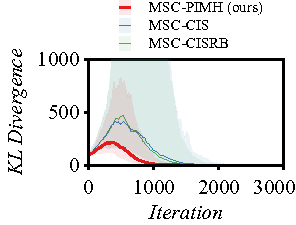
\includegraphics[scale=0.75]{figures/gaussian_01.pdf}
  }
  \subfloat[\(N=2^4\)]{
    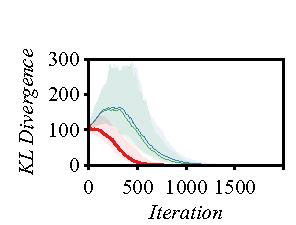
\includegraphics[scale=0.75]{figures/gaussian_02.pdf}
  }
  \subfloat[\(N=2^6\)]{
    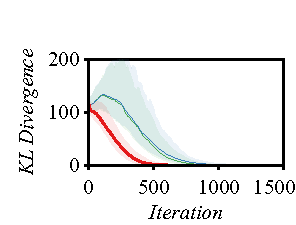
\includegraphics[scale=0.75]{figures/gaussian_03.pdf}
  }
  \caption{100-D isotropic Gaussian example with a varying computational budget \(N\).
    MSC-PIMH converges faster than MSC-CIS and MSC-CISRB regardless of \(N\).
    Also, the convergence of MSC-PIMH becomes more stable/monotonic as \(N\) increases.
    The solid lines and colored regions are the medians and 80\% percentiles computed from 100 repetitions.
  }\label{fig:gaussian}
\end{figure}
%
We perform experiments with a 100-D isotropic multivariate Gaussian distribution.
With Gaussian distributions, convergence can be evaluated exactly since their KL divergence is available in a closed form.
We compare the performance of MSC-PIMH, MSC-CIS, and MSC-CISRB with respect to the \(N\) (number of proposals for MSC-CIS, MSC-CISRB; number of parallel chains for MSC-PIMH).
The results are shown in~\cref{fig:gaussian}.
While MSC-PIMH shows some level of overshoot wih \(N=4\), it shows monotonic convergence with larger \(N\).
On the other hand, both MSC-CIS and MSC-CISRB overshoots even with \(N=64\).
This clearly shows that PIMH enjoys better gradient estimates compared to the CIS kernel.

\section{Numerical Simulation}
We present numerical simulations of our analyses in~\cref{section:bias_variance} and~\cref{section:cis_bias}.
In particular, we visualize the fact that the variance of the CIS kernel can increase with the number of proposals \(N\) when the KL divergence is large, as described in~\eqref{eq:cis_variance_incr}.

\paragraph{Experimental Setup}
We first set the target distribution as \(p\,(z \mid x) = \mathcal{N}(0, 1)\) and the proposal distribution as \(q\,(z; \mu) = \mathcal{N}(\mu, 2)\) with varying mean.
We measure the variance of estimating the score function \(s\,(z, \mu) = \frac{\partial q(\vz; \mu)}{\partial \mu} \) using the CIS, CISRB, and PIMH kernels, given the previous Markov-chain  denoted bystate \(z_{t-1}\) and computational budget \(N\).
For CIS and CISRB, we set a fixed \(z_{t-1}\), while for PIMH, we randomly sample \(N\) samples from \(\vz_{t-1} \sim p\,(z \mid z)\) (we obtained similar trends regardless of the distribution of \(z_{t-1}\)).
The variance is estimated using \(2^{14}\) samples from \(K(\vz_{t-1}, \cdot)\).
We report the variance across varying \(N\) and varying KL divergence between \(q_{\vlambda}(z)\) and \(p\,(\vz\mid\vx)\).
The latter is performed by varying the difference between the mean of the proposal and the target distributions denoted by \(\Delta \mu = \Esub{p(\vz\mid\vx)}{z} - \Esub{q_{\vlambda}}{z} \).

\begin{figure}[H]
  \centering
  \subfloat[\(\Delta \mu = 0\)]{
    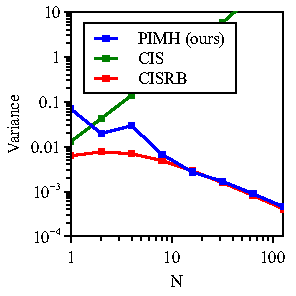
\includegraphics[scale=0.75]{figures/simulations_01.pdf}
  }
  \subfloat[\(\Delta \mu = 2\)]{
    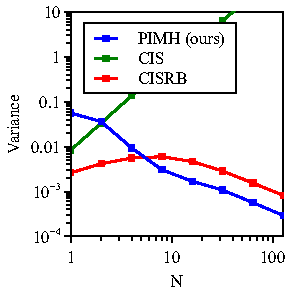
\includegraphics[scale=0.75]{figures/simulations_02.pdf}
  }
  \subfloat[\(\Delta \mu = 4\)]{
    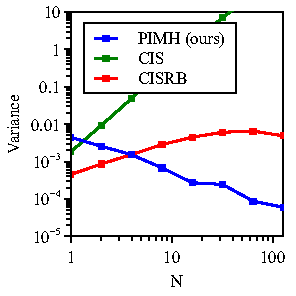
\includegraphics[scale=0.75]{figures/simulations_03.pdf}
  }
  \caption{Conditional variance of different MCMC kernels with varying \(N\) and varying difference between the mean of the target and proposal distributions.
  }\label{fig:simulations}
  \vspace{-0.1in}
\end{figure}

\paragraph{Results Summary}
The results are presented in~\cref{fig:simulations}.
We can see that, when the difference of the mean of the \(p\) and \(q\) is large, the variance of CISRB \textit{increases} with \(N\).
This increasing trend becomes stronger as the KL divergence between \(p\) and \(q\) increases.
While this simulation suggests that CISRB has much smaller variance compared to CIS, our realistic experiments in~\cref{section:eval} did not reveal such levels of performance gains.
Is also visible that PIMH has a slightly larger variance compared to CIS in the small \(N\) regime.
This is due to the higher acceptance rate of the Metropolis-Hastings acceptance ratio used by PIMH compared to Barker's acceptance ratio used by CIS~\citep{peskun_optimum_1973, minh_understanding_2015}.

%%% Local Variables:
%%% TeX-master: "master"
%%% End:
